% Template for ICIP-2015 paper; to be used with:
%          spconf.sty  - ICASSP/ICIP LaTeX style file, and
%          IEEEbib.bst - IEEE bibliography style file.
% --------------------------------------------------------------------------
\documentclass{article}
\usepackage{spconf,amsmath,graphicx}
\usepackage{listings}
\usepackage{float}
\usepackage{pythonhighlight}
% Example definitions.
% --------------------
\def\x{{\mathbf x}}
\def\L{{\cal L}}

% Title.
% ------
\title{Processamento Digital de Imagens - Trabalho 4}
%
% Single address.
% ---------------
\name{Bruna Medeiros da Silva - 16/0048711}
\address{UnB - FGA}
%
% For example:
% ------------
%\address{School\\
%	Department\\
%	Address}
%
% Two addresses (uncomment and modify for two-address case).
% ----------------------------------------------------------
%\twoauthors
%  {A. Author-one, B. Author-two\sthanks{Thanks to XYZ agency for funding.}}
%	{School A-B\\
%	Department A-B\\
%	Address A-B}
%  {C. Author-three, D. Author-four\sthanks{The fourth author performed the work
%	while at ...}}
%	{School C-D\\
%	Department C-D\\
%	Address C-D}
%
\begin{document}
%\ninept
%
\maketitle

%
\section{Questão 1 - Region Labeling Algorithm}
Algoritmos de rotulação de componentes são algoritmos desenvolvidos para detectar a presença de objetos dentro da imagem e identificar suas posições, rotulando-os.

Essa detecção pode ser feita utilizando 3 métodos:

\begin{itemize}
	\item \textbf{\textit{Recursive Tracking}}, que raramente é utilizado;
	\item \textbf{\textit{Parallel Growing}}, que necessita de computação paralela e
	 \item \textbf{\textit{Row-by-Row}}, que faz uso de um algoritmo mais simples e é o mais comumente utilizado.
\end{itemize}

Com isso, a técnica utilizada para o desenvolvimento desse algoritmo, foi pelo método Row-by-Row.

\subsection{Metodologia}
Para chegar ao resultado esperado, a imagem foi percorrida 2 vezes. Para a primeira, onde realiza-se uma primeira rotulação dos componentes, de  foram aplicados os seguintes passos:

\begin{enumerate}
	\item Binarização da imagem, utilizando limiares (\textit{threshold}) de acordo com a necessidade visualizada para cada imagem;
	\item Pré-processamento/Tratamento morfológico da imagem, com o objetivo de preencher buracos;
	\item Percorre-se a imagem de linha em linha, analisando a vizinhança de 8 de cada pixel;
	\item Se o pixel em questão for 1 e vier depois de um zero, será definido como um novo componente, utilizando o menor valor inteiro positivo ainda não utilizado para rotulação;
	\item Se esse mesmo pixel tiver algum vizinho já percorrido com um valor menor que ele, deve-se armazenar o valor mais baixo entre eles, utilizar um dicionário ou algo que relacione os dois identificadores para uma modificação posterior.	
\end{enumerate}

Nesse segundo momento, deve-se percorrer novamente a imagem, linha por linha, para realizar as alterações dos casos de conflito, substituindo sempre os valores mais altos pelos mais baixos.

As principais operações morfológicas utilizadas nessa etapa foram as operações de fechamento,  visando cobrir "rastros" de pixels vazios dentro da imagem. 

Nas Figuras \ref{fig: test1} a \ref{fig: test7}

\begin{figure}[H]
	\label{fig: test1}
	\begin{minipage}[b]{1.0\linewidth}
		\centering
		\centerline{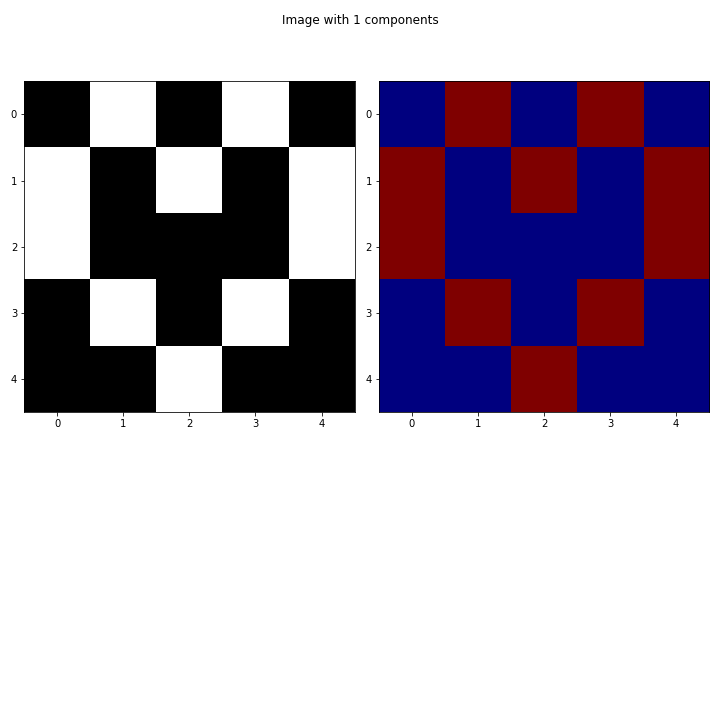
\includegraphics[width=8.5cm]{Figures/test1.png}}
		\vspace{-2.0cm}
		\centerline{Figura de teste 1 do algoritmo de Rotulação de componentes}\medskip	
	\end{minipage}
\end{figure}

\begin{figure}[H]
	\label{fig: test2}
	\begin{minipage}[b]{1.0\linewidth}
		\centering
		\centerline{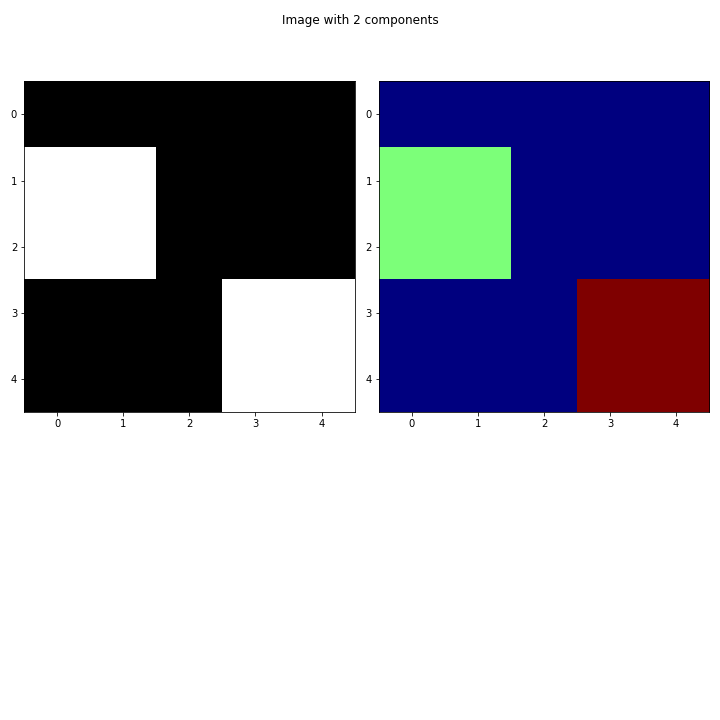
\includegraphics[width=8.5cm]{Figures/test2.png}}
		\vspace{-2.0cm}
		\centerline{Figura de teste 2 do algoritmo de Rotulação de componentes}\medskip	
	\end{minipage}
\end{figure}

\begin{figure}[H]
	\label{fig: test3}
	\begin{minipage}[b]{1.0\linewidth}
		\centering
		\centerline{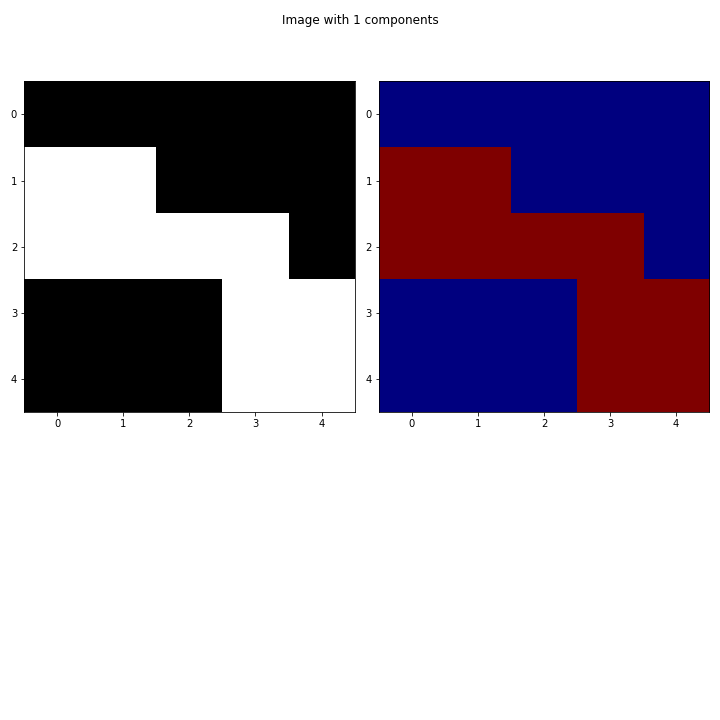
\includegraphics[width=8.5cm]{Figures/test3.png}}
		\vspace{-2.0cm}
		\centerline{Figura de teste 3 do algoritmo de Rotulação de componentes}\medskip	
	\end{minipage}
\end{figure}

\begin{figure}[H]
	\label{fig: test4}
	\begin{minipage}[b]{1.0\linewidth}
		\centering
		\centerline{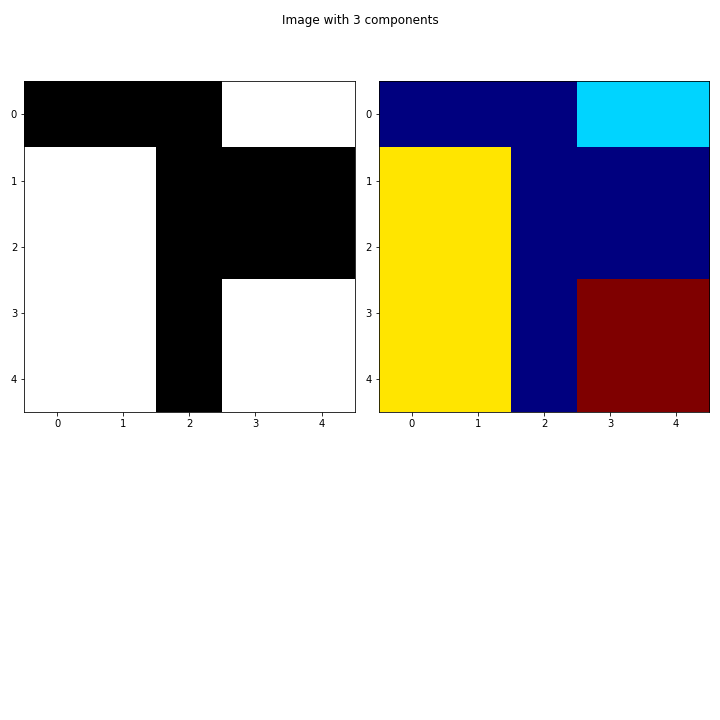
\includegraphics[width=8.5cm]{Figures/test4.png}}
		\vspace{-2.0cm}
		\centerline{Figura de teste 4 do algoritmo de Rotulação de componentes}\medskip	
	\end{minipage}
\end{figure}

\begin{figure}[H]
	\label{fig: test5}
	\begin{minipage}[b]{1.0\linewidth}
		\centering
		\centerline{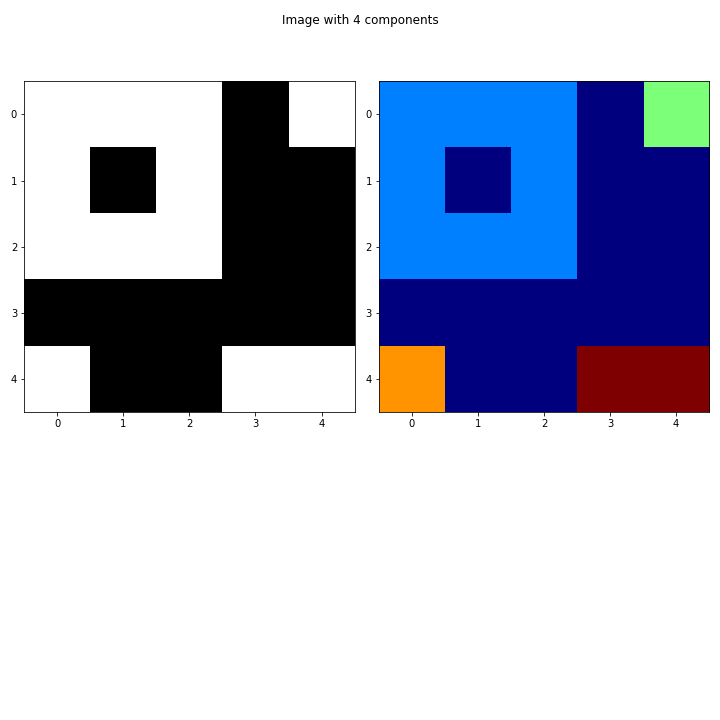
\includegraphics[width=8.5cm]{Figures/test5.png}}
		\vspace{-2.0cm}
		\centerline{Figura de teste 5 do algoritmo de Rotulação de componentes}\medskip	
	\end{minipage}
\end{figure}

\begin{figure}[H]
	\label{fig: test6}
	\begin{minipage}[b]{1.0\linewidth}
		\centering
		\centerline{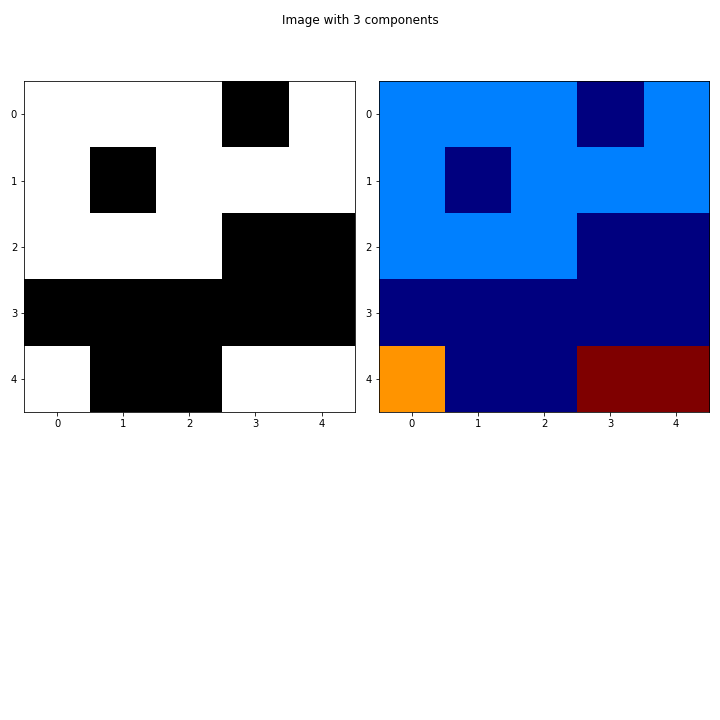
\includegraphics[width=8.5cm]{Figures/test6.png}}
		\vspace{-2.0cm}
		\centerline{Figura de teste 6 do algoritmo de Rotulação de componentes}\medskip	
	\end{minipage}
\end{figure}

\begin{figure}[H]
	\label{fig: test7}
	\begin{minipage}[b]{1.0\linewidth}
		\centering
		\centerline{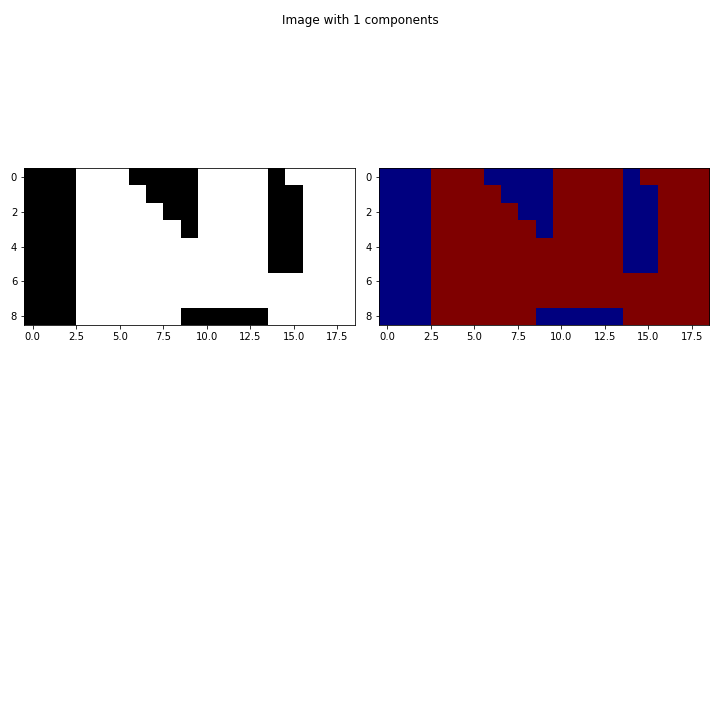
\includegraphics[width=8.5cm]{Figures/test7.png}}
		\vspace{-2.0cm}
		\centerline{Figura de teste 7 do algoritmo de Rotulação de componentes}\medskip	
	\end{minipage}
\end{figure}

A segunda vez em que percorre-se a imagem, fazesse no intuito de realizar as substituições nos casos de conflito, substituindo sempre o valor mais alto pelo mais baixo dentro da vizinhança do pixel. Para realizar essa operação é utilizada uma condicional dentro dos loops que percorrem as colunas e linhas da imagem, verificando o valor dos pixels e substituindo-os. 

Na detecção e separação dos objetos da imagem, visto que cada mancha possui seu próprio número identificador (o valor dos pixels atribuído) , obteve-se os extremos em X e em Y com esse dado valor, gerando uma imagem retangular que contendo toda a mancha. 

Nesse ponto foram realizados outros processos morfológicos, tais como  abertura e compressão, com o intuito de remover pequenos componentes que atrapalhariam a detecção correta dos limites da imagem. 

Para identificar os resultados alcançado foi muito melhor realizando um processo de detecção de bordas, inversão da imagem e aplicando novamente o algoritmo de detecção de componentes sobre o resultado, obtendo uma maior taxa de acertos quando comparado a casos utilizando apenas processamento morfológico de diversos tipos.  Com isso, a quantidade de manchas detectadas passa a ser a quantidade de buracos existentes. 

Para contabilizar a porcentagem do componente composto por buracos, construiu-se um algoritmo que novamente detecta as bordas de cada linha da imagem, considerando os pontos pretos (zeros) nesse intervalo como buracos. Essa quantidade será somada, linha a linha, e divida no final pela quantidade total de pixels, que também é somada a cada iteração. O valor obtido será considerado a porcentagem de buracos dentro de cada mancha.





\begin{figure}[H]
	\label{fig:img_clown}
	\begin{minipage}[b]{1.0\linewidth}
		\centering
		\centerline{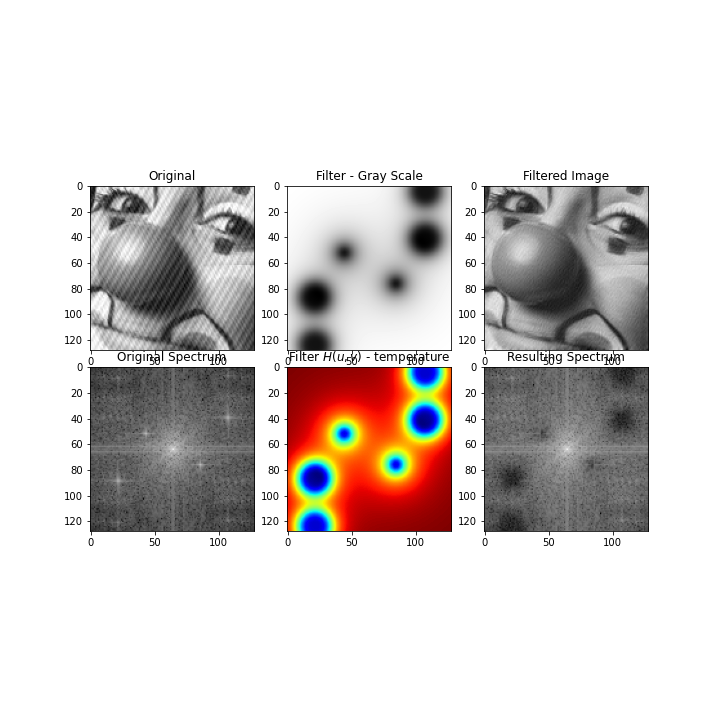
\includegraphics[width=8.5cm]{Figures/filtered_clown}}
		\vspace{-2.0cm}
		\centerline{Resultado da aplicação do filtro Notch na}
		\centerline{Figura \textit{clown\_notch.jpg}}\medskip	
	\end{minipage}
\end{figure}




% -----------------------------------------------------------------
%\vfill
%\pagebreak
\newpage
\onecolumn
\section{Códigos}

\subsection{Filtragem Homomórfica}
\label{cod:homomorfic}
\begin{python}
from scipy import signal
from numpy.fft import fft2, ifft2, fftshift, ifftshift

## HP: gamma_L < 1, gamma_H > 1
## Reduce ilumination component and increase refraction component
## P >= M
## Q >= N

def img_filtering(image, gamma_H = 2, gamma_L = 0.25, c = 1, D_0 = 80):
	fft_image = fftshift(fft2(image))
	
	M, N = fft_image.shape
	P = M
	Q = N
	H = np.zeros(fft_image.shape)
	
	for u in range(M):
		for v in range(N):
			D = ((u - (P/2))**2 + (v - (Q/2))**2)**(1 / 2)
			H[u][v] = (gamma_H - gamma_L) * (1 - np.exp(- c * (D**2 / (D_0**2)))) + gamma_L
	filt_fft_img = fft_image * H
	filtered_img = ifft2(ifftshift(filt_fft_img))
	return filtered_img, H
	
def homomorfic_filter(image, gamma_H = 2, gamma_L = 0.25, c = 1, D_0 = 80, tol = 1e-3):
	if(len(image.shape) > 2):
		image = cv2.cvtColor(image, cv2.COLOR_BGR2GRAY)
	
	new_image = np.zeros(image.shape).astype(np.float)
	freq_filter = np.zeros(image.shape)
	
	log_image = image + tol
	log_image = np.log(log_image)    
	
	img_filtered, freq_filter = img_filtering(log_image, gamma_H = gamma_H,  
																						gamma_L = gamma_L, c = c, D_0 = D_0)
	img_filtered = np.exp(np.real(img_filtered))
	img_filtered = img_filtered * 255 / img_filtered.max()
	
	new_image = image + img_filtered
	new_image = np.floor(new_image * 255 / new_image.max())

	return new_image.astype(np.uint8), freq_filter, img_filtered


def plot_results_1(original_img, freq_filter, new_img, added_img, hspace = -0.5, tol = 1e-3, fig_name = 'fig_pdi'):
	fig, axs = plt.subplots(2, 3, figsize = [15, 15])
	fig.subplots_adjust(hspace = hspace)
	
	axs[0][0].imshow(original_img, cmap = 'gray', vmin = 0, vmax = 255)
	axs[0][0].set_title('Original')
	axs[0][1].set_title('Filtered Image (gray)')
	axs[0][1].imshow(added_img, cmap = 'gray', vmin = 0, vmax = 255)
	axs[0][2].set_title('Result')
	axs[0][2].imshow(new_img, cmap = 'gray', vmin = 0, vmax = 255)
	axs[1][0].set_title('Original Spectrum')
	axs[1][0].imshow(20*np.log10(np.abs(fftshift(fft2(original_img))) + tol), cmap = 'gray')
	axs[1][1].set_title('Homomorfic Filter $H(u, v)$')
	axs[1][1].imshow(20*np.log10(freq_filter), cmap = 'jet')
	axs[1][2].set_title('Resulting Spectrum')
	axs[1][2].imshow(20*np.log10(np.abs(fftshift(fft2(new_img))) + tol), cmap = 'gray')
	plt.savefig(fig_name+'.png')
\end{python}

\newpage

\subsection{Filtragem homomórfica da imagem mussels\_cave\_050.JPG}
\label{cod:mussels}
\begin{python}img_mussels = cv2.imread("imagens_5_freq/mussels_cave_050.JPG")
	plt.imshow(img_mussels)
	if(len(img_mussels.shape) > 2):
		img_mussels = cv2.cvtColor(img_mussels, cv2.COLOR_BGR2GRAY)
		
		
filtered_mussels, filter_mussels, added_mussels = homomorfic_filter(img_mussels, 
gamma_H = 2, gamma_L = 0.25, c = 3, D_0 = 30)

plot_results_1(img_mussels, 
					filter_mussels, 
					filtered_mussels, 
					added_mussels, 
					fig_name = 'q1_mussels')
\end{python}


\subsection{Filtragem homomórfica da imagem shelter\_homomorphic.bmp}
\label{cod:shelter}
\begin{python}
img_shelter = cv2.imread("imagens_5_freq/shelter_homomorphic.bmp")

if(len(img_shelter.shape) > 2):
	img_shelter = cv2.cvtColor(img_shelter, cv2.COLOR_BGR2GRAY)
	
plt.imshow(img_shelter, cmap = 'gray')

filtered_shelter, filter_shelter, added_shelter = homomorfic_filter(img_shelter, 
gamma_H = 2, gamma_L = 0.25, c = 8, D_0 = 20)

plot_results_1(img_shelter, 
				filter_shelter, 
				filtered_shelter, 
				added_shelter,
				hspace = - 0.3,
				fig_name = 'q1_shelter')
\end{python}

\subsection{Filtragem homomórfica da imagem mussels\_cave\_050.JPG}
\label{cod:seal}
\begin{python}
img_seal = cv2.imread("imagens_5_freq/The_Seventh_Seal_1.jpg")

if(len(img_seal.shape) > 2):
	img_seal = cv2.cvtColor(img_seal, cv2.COLOR_BGR2GRAY)

plt.imshow(img_seal, cmap = 'gray')

filtered_seal, filter_seal, added_seal = homomorfic_filter(img_seal, 
gamma_H = 1.5, gamma_L = 0.25, c = 5, D_0 = 15)

plot_results_1(img_seal, 
filter_seal, 
filtered_seal, 
added_seal,
hspace = - 0.6,
fig_name = 'q1_seal')
\end{python}


\newpage
\subsection{Filtragem de ruíde periódico com Filtro Notch}
\label{cod:notch}
\begin{python}
def notch_filter(img, D_0 = 5, uk = -80, vk = 30, n = 1, dist_y = 40, dist_x = 0, plot = True, 
								 hspace = -0.5, filt_zeros = False, fig_name = 'fig_pdi'):
								 
	if(len(img.shape) > 2):
		img = cv2.cvtColor(img, cv2.COLOR_BGR2GRAY)
	
	fft_img = fftshift(fft2(img)) 
	M, N = fft_img.shape
	H = np.zeros([M, N])
	final_H = np.ones([M, N])
	u, v = np.meshgrid(range(M), range(N), sparse=False, indexing='ij');
	
	for k in range(n):    
		Dk  = np.sqrt((u - (M/2) - uk)**2 + (v - (N/2) - vk)**2)
		D_k = np.sqrt((u - (M/2) + uk)**2 + (v - (N/2) + vk)**2)
		Dk[Dk == 0] = 0.000001 		# avoid divisions by zero
		D_k[D_k == 0] = 0.000001 	# avoid divisions by zero
		
		H = (1 / (1 + (D_0/Dk)**(2*n))) * (1 / (1 + (D_0/D_k)**(2*n)))
		final_H = final_H * H
		
		if(((uk + dist_y) != 0 or filt_zeros) and ((vk + dist_x) != 0 or (uk + dist_y != 0))):
			uk = uk + dist_y
		else:
			uk = uk + (2 * dist_y)
		
		if(((vk + dist_x) != 0 or filt_zeros) and ((vk + dist_x) != 0 or (uk != 0))):
			vk = vk + dist_x
		else:
			vk = vk + (2 * dist_x)
		
	filtered_fft_img = fft_img * final_H
	filtered_img = abs(ifft2(ifftshift(filtered_fft_img)))
	filtered_img = (filtered_img * 255 / filtered_img.max()).astype(np.uint8)
	
	if(plot):
		plot_results_2(img, 
					final_H, 
					filtered_img, 
					hspace = hspace,
					fig_name = fig_name)
	
	return filtered_img, final_H

def plot_results_2(original_img, freq_filter, new_img, hspace = -0.5, tol = 1e-3, fig_name = 'fig_pdi'):
	if(len(original_img.shape) > 2):
		original_img = cv2.cvtColor(original_img, cv2.COLOR_BGR2GRAY)
	
	fig, axs = plt.subplots(2, 3, figsize = [10, 10])
	fig.subplots_adjust(hspace = hspace)
	
	axs[0][0].imshow(original_img, cmap = 'gray', vmin = 0, vmax = 255)
	axs[0][0].set_title('Original')
	axs[0][1].set_title('Filter - Gray Scale')
	axs[0][1].imshow(20*np.log10(freq_filter), cmap = 'gray')
	axs[0][2].set_title('Filtered Image')
	axs[0][2].imshow(new_img, cmap = 'gray', vmin = 0, vmax = 255)
	axs[1][0].set_title('Original Spectrum')
	axs[1][0].imshow(20*np.log10(np.abs(fftshift(fft2(original_img))) + tol), cmap = 'gray')
	axs[1][1].set_title('Filter $H(u, v)$ - temperature')
	axs[1][1].imshow(20*np.log10(freq_filter), cmap = 'jet')
	axs[1][2].set_title('Resulting Spectrum')
	axs[1][2].imshow(20*np.log10(np.abs(fftshift(fft2(new_img))) + tol), cmap = 'gray')
	
	plt.savefig(fig_name + '.png')
\end{python}


\newpage
\subsection{Filtragem Notch da imagem clown\_notch.jpg}
\label{cod:clown}
\begin{python}
clown_img = cv2.imread('imagens_5_freq/clown_notch.jpg')

if(len(clown_img.shape) > 2):
	clown_img = cv2.cvtColor(clown_img, cv2.COLOR_BGR2GRAY)

filter_clown = np.zeros(clown_img.shape)

filtered_clown,filter_tmp = notch_filter(clown_img, uk = -12, vk = -20, D_0 = 10, n = 1, dist_y = 40, dist_x = 0, plot = False)
filter_clown = filter_clown + filter_tmp 

filtered_clown,filter_tmp = notch_filter(filtered_clown, uk = -60, vk = 43,  D_0 = 15, n = 2, dist_y = 37, dist_x = 0, hspace = - 0.3, plot = False)
filter_clown = filter_clown + filter_tmp

filter_clown = filter_clown * 255 / filter_clown.max()
plot_results_2(clown_img, filter_clown, filtered_clown, fig_name = 'filtered_clown')
\end{python}

\subsection{Filtragem Notch da imagem Fig0464(a)(car\_75DPI\_Moire).tif}
\label{cod:car}
\begin{python}
car_img = cv2.imread('imagens_5_freq/Fig0464(a)(car_75DPI_Moire).tif')

filtered_car,_ = notch_filter(car_img, uk = -80, vk = 30, D_0 = 10, n = 4, dist_y = 40, dist_x = 0, hspace = 0, fig_name = 'filtered_car')
\end{python}


\subsection{Filtragem Notch da imagem halftone.png}
\label{cod:halftone}
\begin{python}
halftone_img = cv2.imread('imagens_5_freq/halftone.png')

filtered_halftone, filter_halftone = notch_filter(halftone_img, uk = -345, vk = -100, D_0 = 20, n = 6, 
dist_y = 135, dist_x = 0, hspace = -0.6, filt_zeros = True, plot = False)
filtered_halftone, tmp_filter = notch_filter(filtered_halftone, uk = -345, vk = -100, D_0 = 20, n = 6, 
dist_y = 135, dist_x = 0, hspace = -0.6, filt_zeros = True, plot = False)
filter_halftone = filter_halftone + tmp_filter


filtered_halftone, tmp_filter = notch_filter(filtered_halftone, uk = -270, vk = -200, D_0 = 20, n = 5, 
dist_y = 135, dist_x = 0, hspace = -0.6, filt_zeros = True, plot = False)
filter_halftone = filter_halftone + tmp_filter


filtered_halftone, tmp_filter = notch_filter(filtered_halftone, uk = -345, vk = -300, D_0 = 20, n = 6, 
dist_y = 135, dist_x = 0, hspace = -0.6, filt_zeros = True, plot = False)
filter_halftone = filter_halftone + tmp_filter


filtered_halftone, tmp_filter = notch_filter(filtered_halftone, uk = -270, vk = -400, D_0 = 20, n = 5, 
dist_y = 135, dist_x = 0, hspace = -0.6, filt_zeros = True, plot = False)
filter_halftone = filter_halftone + tmp_filter


filtered_halftone, tmp_filter = notch_filter(filtered_halftone, uk = -270, vk = 0, D_0 = 20, n = 5, 
dist_y = 135, dist_x = 0, hspace = -0.6, filt_zeros = True, plot = False)
filter_halftone = filter_halftone + tmp_filter

filter_halftone = (np.round(filter_halftone * 255 / filter_halftone.max()))


plot_results_2(halftone_img, filter_halftone, filtered_halftone, fig_name = 'filtered_halftone')
\end{python}

\end{document}
